\documentclass{article}
\usepackage{amsmath}
\usepackage{tikz}
\raggedright
\pagestyle{empty}
\usepackage[margin = 0.5in]{geometry}
\begin{document}

Name \makebox[2.5in]{\hrulefill} \quad Period \makebox[0.35in]{\hrulefill}    \hfill Honors PreCalc P-Set

\subsubsection*{Basic Set Theory and Interval Notation \hfill \makebox[0.35in]{\hrulefill} / 10}

\newline\\

You are given a form of a set of real numbers as either an interval, set-builder notation, or the graph. Express it in the other two possible ways.
\begin{flalign*}
1.  \quad   &   (-3,\ 5)    &
2.  \quad   &   x \leq 2    &
3.  \quad   &   
\raisebox{-0.35cm}{
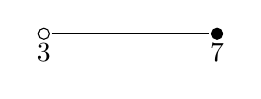
\begin{tikzpicture}
\draw (0,0)--(2,0);
\draw (-0.1,0) circle (2pt);
\draw [fill=black] (2.1,0) circle (2pt);
\node at (-0.1,0) [anchor = north] {3};
\node at (2.1,0) [anchor = north] {7};
\end{tikzpicture}}   &&\\[1.5in]
4.  \quad   &   x > -1  &
5.  \quad   &   
\raisebox{-0.35cm}{
\begin{tikzpicture}
\draw [->, > = stealth] (0,0)--(2,0);
\draw [fill=black] (-0.1,0) circle (2pt);
\node at (-0.1,0) [anchor = north] {$-1$};
\end{tikzpicture}}   &
6.  \quad   &   (-\infty, \ 6]  &&\\[1.5in]
7.  \quad   &   
\raisebox{-0.35cm}{
\begin{tikzpicture}
\draw [->, >=stealth] (2,0) -- (0,0);
\draw (2.1,0) circle (2pt);
\node at (2.1,0) [anchor=north] {7};
\end{tikzpicture}}
&
8.  \quad   &   (5, \ \infty)   &
9.  \quad   &   x \geq 9    &&\\[1.25in]
\end{flalign*}

Write each of the following in interval notation and graph.
\begin{flalign*}
10. \quad   &   x < 8 \text{ or } x \geq 11    & 
11.  \quad   &   -2 < x \leq 6   &
12. \quad   &   x \leq -2 \text{ or } x > 9   &&\\[1.5in]
13. \quad   &   x \neq 3    &
14. \quad   &   x \neq -6, \ 5  &
15. \quad   &   x \neq 0, \pm 4 &&\\
\end{flalign*}

\newpage


Many word processing programs such as Microsoft Word and Google Docs have built-in mathematical text capabilities (making your document easily readable). 
\newline\\


Use either of these programs (or another) to write the following formulas or equations. If they are already available, see if you can write them on your own.
\begin{flalign*}
16. \quad   &    \sin^2 \theta + \cos^2 \theta = 1  &
17. \quad   &   x = \dfrac{-b \pm \sqrt{b^2-4ac}}{2a} &
18. \quad   &   P(x) = \dfrac{1}{\sigma \sqrt{2\pi}}e^{\frac{-(x-\mu)^2}{2\sigma^2}}    &&\\  
\end{flalign*}


19. If you \emph{really} want to take it to the next level, learn the mark-up language \LaTeX{}. It is what I use to create just about everything I hand you in this course (including this problem set).
\newline\\

It's free, but there is a pretty big learning curve to it. So don't be surprised if it takes you a long time to learn it. However, you'll find it far superior to anything on the market for technical writing once you start getting the hang of it.
\newline\\


I recommend www.overleaf.com to get started.


\newpage


\textbf{Sets of Real Numbers KEY}

\begin{enumerate}
    \item $-3 < x < 5$  \qquad 
    \raisebox{-0.25cm}{
    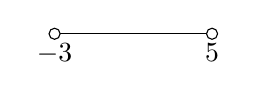
\begin{tikzpicture}
    \draw (0,0) -- (2,0);
    \draw [fill = white] (0,0) circle (2pt);
    \node at (0,0) [anchor = north] {$-3$};
    \draw [fill = white] (2,0) circle (2pt);
    \node at (2,0) [anchor = north] {$5$};
    \end{tikzpicture}}  \\[0.25in]
    
    \item $(-\infty, 2]$    \qquad
    \raisebox{-0.25cm}{
    \begin{tikzpicture}
    \draw [<-, >=stealth] (0,0) -- (2,0);
    % \draw [fill = white] (0,0) circle (2pt);
    % \node at (0,0) [anchor = north] {$-3$};
    \draw [fill = black] (2,0) circle (2pt);
    \node at (2,0) [anchor = north] {$2$};
    \end{tikzpicture}}  \\[0.25in]
    
    \item $(3, 7] \qquad 3 < x \leq 7$  \\[0.25in]
    
    \item $(-1, \infty)$    \qquad
    \raisebox{-0.25cm}{
    \begin{tikzpicture}
    \draw [->, >=stealth] (0,0) -- (2,0);
    \draw [fill = white] (0,0) circle (2pt);
    \node at (0,0) [anchor = north] {$-1$};
    % \draw [fill = black] (2,0) circle (2pt);
    % \node at (2,0) [anchor = north] {$2$};
    \end{tikzpicture}}  \\[0.25in]    
    
    \item $[-1, \infty) \qquad x \geq -1$   \\[0.25in]
    
    \item $x \leq 6$    \qquad
    \raisebox{-0.25cm}{
    \begin{tikzpicture}
    \draw [<-, >=stealth] (0,0) -- (2,0);
    % \draw [fill = white] (0,0) circle (2pt);
    % \node at (0,0) [anchor = north] {$-3$};
    \draw [fill = black] (2,0) circle (2pt);
    \node at (2,0) [anchor = north] {$6$};
    \end{tikzpicture}}  \\[0.25in]   
    
    \item $x < 7 \qquad (-\infty, 7)$   \\[0.25in]
    
    \item $x > 5$   \qquad
    \raisebox{-0.25cm}{
    \begin{tikzpicture}
    \draw [->, >=stealth] (0,0) -- (2,0);
    \draw [fill = white] (0,0) circle (2pt);
    \node at (0,0) [anchor = north] {$5$};
    % \draw [fill = black] (2,0) circle (2pt);
    % \node at (2,0) [anchor = north] {$2$};
    \end{tikzpicture}}  \\[0.25in]
    
    \item $[9, \infty)$   \qquad
    \raisebox{-0.25cm}{
    \begin{tikzpicture}
    \draw [->, >=stealth] (0,0) -- (2,0);
    \draw [fill = black] (0,0) circle (2pt);
    \node at (0,0) [anchor = north] {$9$};
    % \draw [fill = black] (2,0) circle (2pt);
    % \node at (2,0) [anchor = north] {$2$};
    \end{tikzpicture}}  \\[0.25in] 
    
    \item $(-\infty, 8) \cup [11, \infty)$  \qquad
    \raisebox{-0.25cm}{
    \begin{tikzpicture}
    % \draw [->, >=stealth] (0,0) -- (2,0);
    \draw [->, >=stealth] (0,0) -- (-2,0);
    \draw [fill = white] (0,0) circle (2pt);
    \node at (0,0) [anchor = north] {$8$};
    \draw [->, >=stealth] (2,0) -- (4,0);
    \draw [fill = black] (2,0) circle (2pt);
    \node at (2,0) [anchor = north] {$11$};
    \end{tikzpicture}}  \\[0.25in] 
    
    \item $(-2, 6]$ \qquad
    \raisebox{-0.25cm}{
    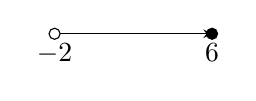
\begin{tikzpicture}
    \draw [->, >=stealth] (0,0) -- (2,0);
    \draw [fill = white] (0,0) circle (2pt);
    \node at (0,0) [anchor = north] {$-2$};
    \draw [fill = black] (2,0) circle (2pt);
    \node at (2,0) [anchor = north] {$6$};
    \end{tikzpicture}}  \\[0.25in] 
    
    \item $(-\infty, -2] \cup (9, \infty)$  \qquad
    \raisebox{-0.25cm}{
    \begin{tikzpicture}
    % \draw [->, >=stealth] (0,0) -- (2,0);
    \draw [->, >=stealth] (0,0) -- (-2,0);
    \draw [fill = black] (0,0) circle (2pt);
    \node at (0,0) [anchor = north] {$-2$};
    \draw [->, >=stealth] (2,0) -- (4,0);
    \draw [fill = white] (2,0) circle (2pt);
    \node at (2,0) [anchor = north] {$9$};
    \end{tikzpicture}}  \\[0.25in] 
    
    \item $(-\infty, 3) \cup (3, \infty)$   \qquad
    \raisebox{-0.25cm}{
    \begin{tikzpicture}
    \draw [<->, >=stealth] (-2,0) -- (2,0);
    \draw [fill = white] (0,0) circle (2pt);
    \node at (0,0) [anchor = north] {$3$};
    \end{tikzpicture}}  \\[0.25in] 
    
    \item $(-\infty, -6) \cup (-6, 5) \cup (5, \infty)$ \qquad
    \raisebox{-0.25cm}{
    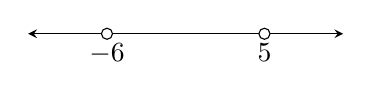
\begin{tikzpicture}
    \draw [<->, >=stealth] (-2,0) -- (2,0);
    \draw [fill = white] (-1,0) circle (2pt);
    \node at (-1,0) [anchor = north] {$-6$};
    \draw [fill = white] (1,0) circle (2pt);
    \node at (1,0) [anchor = north] {$5$};
    \end{tikzpicture}}  \\[0.25in]
    
    \item $(-\infty, -4) \cup (-4, 0) \cup (0, 4) \cup (4, \infty)$ \qquad
    \raisebox{-0.25cm}{
    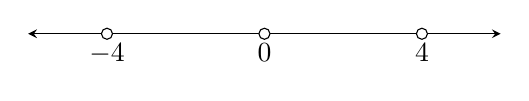
\begin{tikzpicture}
    \draw [<->, >=stealth] (-3,0) -- (3,0);
    \draw [fill = white] (-2,0) circle (2pt);
    \node at (-2,0) [anchor = north] {$-4$};
    \draw [fill = white] (0,0) circle (2pt);
    \node at (0,0) [anchor = north] {$0$};
    \draw [fill = white] (2,0) circle (2pt);
    \node at (2,0) [anchor = north] {$4$};
    \end{tikzpicture}}  \\[0.25in]    
    
    
    
    
    
\end{enumerate}




\end{document}
